\chapter{Laboratorio 2}
\section{Introduzione}
Nell'esperienza di laboratorio precedente, si è realizzato un circuito a guadagno unitario, che realizza una funzione di buffer replicando il segnale in ingresso sull'uscita. Inoltre, esso ha anche una funzione di disaccoppiamento tra ingresso e uscita, con una resistenza di ingresso tendente ad infinito e una resistenza di uscita tendente a zero. 

In questa esperienza di laboratorio, si sono inizialmente effettuate ulteriori misure sul circuito \textit{emitter follower} per poi realizzare una versione \textit{single-ended} dell'\textit{emitter follower}.

\section{Grafico ingresso-uscita \textit{emitter follower}}
Di seguito vengono riportati i risultati delle misure effettuate sul circuito precedentemente realizzato. In ingresso al circuito è stato applicato un segnale sinusoidale con frequenza pari a \SI{1}{\kilo\hertz} e tensione picco-picco variabile da \SI{0.5}{\volt} a \SI{5}{\volt} con step di \SI{0.5}{\volt}. Sono state poi misurate le tensioni picco-picco in ingresso Vpp\sub{i} e in sucita Vpp\sub{o} al circuito grazie alle funzioni integrate dell'oscilloscopio. Per rendere stabile il valore della misura ricavata dall'oscilloscopio, è stato selezionato un filtro a \SI{20}{\mega\hertz} sugli ingressi dell'oscilloscopio e sono state effettuate delle medie (di 6
 campioni) sui segnali. In questo modo è stato possibile ottenere un segnale più pulito da disturbi e rumore (\Fig\ref{fig:emitterfollwer_misurepiccopicco}).
\begin{table}[h!]
	\centering
	\begin{tabular}{c|c}
		\hline
		Vpp\sub{i} [V] & Vpp\sub{o} [V]\\ \hline
		0.509 & 0.491 \\ \hline
		1.019 & 0.984 \\ \hline
		1.502 & 1.476 \\ \hline
		2.080 & 1.994 \\ \hline
		2.565 & 2.474 \\ \hline
		3.037 & 2.962 \\ \hline
		3.524 & 3.459 \\ \hline
		4.022 & 3.967 \\ \hline
		4.606 & 4.470 \\ \hline
		5.089 & 4.945 \\ \hline
	\end{tabular}
\end{table}
\begin{figure}[h!]
	\centering
	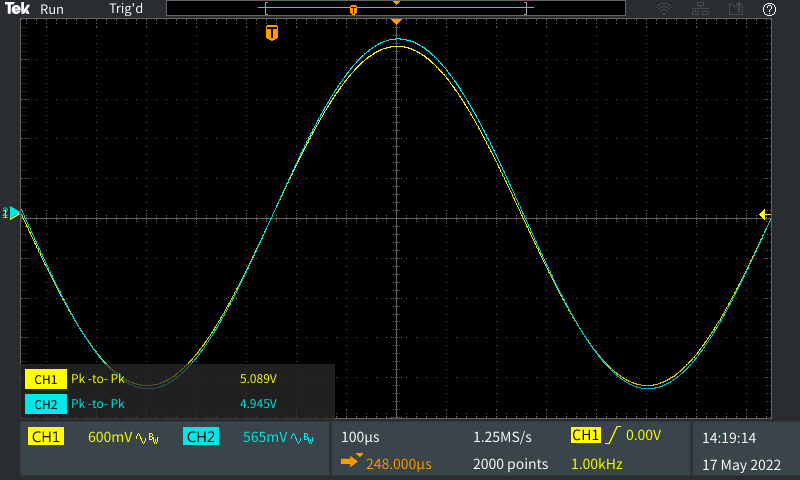
\includegraphics[width=0.7\linewidth]{./ImageFiles/Laboratorio 2/TEK00012}
	\caption{Misurazione della tensione picco-picco del segnale in ingresso (CH1) e in uscita (CH2) con i relativi valori picco-picco misurati dall'oscilloscopio.}
	\label{fig:emitterfollwer_misurepiccopicco}
\end{figure}
\todo{c'è un pezzo su modello equivalente del circuito  non so cosa è}
Come si può notare dalla tabella, il valore del guadagno del circuito è leggermente inferiore a uno. Cerchiamo di quantificare in modo quantitativo quanto il guadagno effettivo del circuito si discosta dal valore teorico unitario. Per fare ciò, rappresentiamo su un grafico il valore picco-picco di tensione misurato all'uscita del circuito in funzione della tensione in ingresso (valori riportati nella tabella precedente). Successivamente, eseguiamo un'interpolazione lineare della retta $y=a+bx$ che approssimi i valori ottenuti. Idealmente, vorremmo ottenere $a=1$ e $b=0$. Infatti, il coefficiente angolare della retta rappresenta il guadagno del circuito, mentre l'intercetta un eventuale offset.

Nella figura \ref{fig:emitterfollwer_inout} viene mostrato il risultato della retta interpolata sui dati stimata grazie alla funzione \textit{fitlm} offerta da Matlab. La retta identificata è $Vpp_o=-0.009+0.977*Vpp_i$. Come si poteva già intuire dalla tabella, abbiamo un guadagno leggermente inferiore a uno ma con un valore molto prossimo.
\begin{figure}[h!]
	\centering
	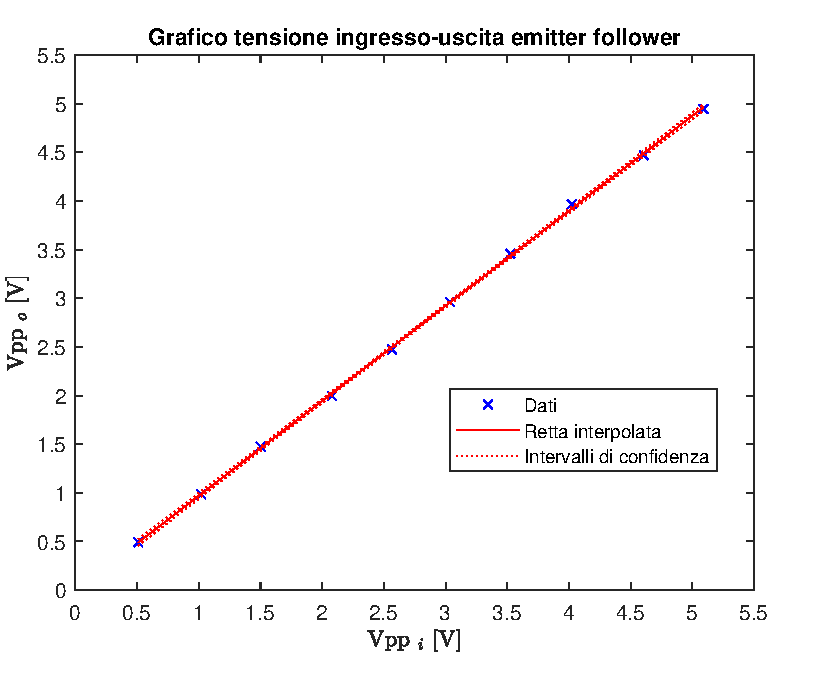
\includegraphics[width=0.7\linewidth]{./OtherFiles/Laboratorio 2/emitter follower-ingresso_uscita}
	\caption{Grafico ingresso-uscita del circuito emitter-follower.}
	\label{fig:emitterfollwer_inout}
\end{figure}

\section{Emitter follower single-ended: prima versione}
Si vuole ora modificare il circuito precedente in modo da alimentarlo tra alimentazione positiva e massa, senza la necessità di utilizzare una alimentazione negativa, realizzando il seguente circuito:
\begin{figure}[h!]
	\centering
	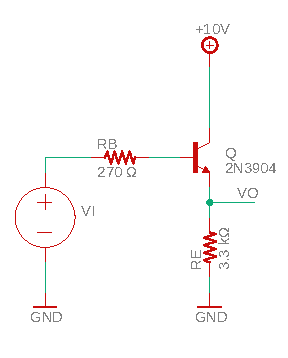
\includegraphics[width=0.4\linewidth]{./OtherFiles/Laboratorio 2/emitter follower}
	\caption{Schematico del circuito emitter follower single-ended.}
	\label{fig:emitterfollwer_se}
\end{figure}
Tuttavia, alimentando questo circuito e applicando una tensione in ingresso V\sub{i} con frequenza di \SI{1}{\kilo\hertz} e tensione picco-picco di \SI{4}{\volt}, il circuito non funziona. Analizziamo il punto di lavoro stazionario (\Fig\ref{fig:emitterfollwer_se_DC}).
\begin{figure}[h!]
	\centering
	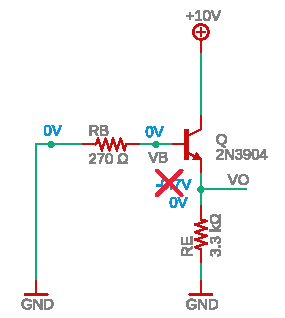
\includegraphics[width=0.4\linewidth]{./OtherFiles/Laboratorio 2/emitter follower_punto di lavoro-printout}
	\caption{Analisi punto di lavoro del circuito emitter follower single-ended.}
	\label{fig:emitterfollwer_se_DC}
\end{figure}
Supponiamo che il transistor sia in zona attiva diretta e con $\beta\to\infty$, con corrente di base nulla. Allora la tensione al nodo V\sub{B} è di \SI{0}{\volt}, poiché non c'è caduta di potenziale in una resistenza attraversata da corrente nulla. Dalle ipotesi fatte, se ne deduce che la tensione al nodo V\sub{o} dovrebbe essere pari a \SI{-0.7}{\volt} (caduta di tensione giunzione base-emettitore). Tuttavia, se così fosse, nella resistenza R\sub{E} scorrerebbe una corrente da massa verso V\sub{o}, in quanto ci sarebbe una differenza di potenziale ai capi della resistenza. Questo però non è possibile: infatti, la corrente dovrebbe poi entrare nel transistor dall'emettitore. Per costruzione, non è però possibile avere una corrente entrante nell'emettitore di un transistor bipolare. Per questo motivo, l'unica soluzione ammissibile è che la corrente che attraversa la resistenza sia nulla e che il circuito sia spento: il nodo V\sub{o} di trova a una tensione di \SI{0}{\volt}. 

Tuttavia, quando applichiamo un segnale alla base con ampiezza maggiore di \SI{0.7}{\volt}, il circuito si accende (\Fig\ref{fig:emitterfollwer_se_statocircuito}). Infatti, il nodo V\sub{o} si porta a una tensione maggiore di \SI{0}{\volt} e il transistor è polarizzato correttamente.
\begin{figure}[h!]
	\centering
	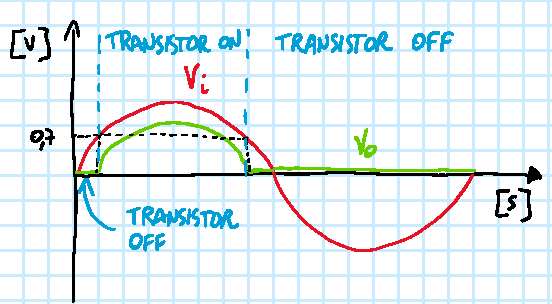
\includegraphics[width=0.7\linewidth]{./ImageFiles/Laboratorio 2/emitter follower errore soglia}
	\caption{Rappresentazione dello stato del circuito in funzione della tensione in ingresso.}
	\label{fig:emitterfollwer_se_statocircuito}
\end{figure}

Questo comportamento è stato verificato sul circuito reale. In figura \ref{fig:emitterfollwer_se_errore} si riportano le misure effettuate.
\begin{figure}[h!]
	\centering
	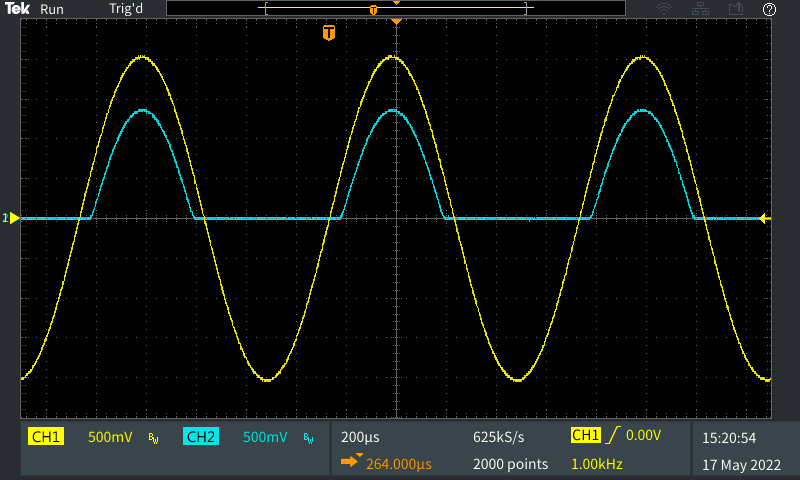
\includegraphics[width=0.7\linewidth]{./ImageFiles/Laboratorio 2/TEK00020}
	\caption{Misurazione della tensione in ingresso (CH1) e in uscita (CH2) del circuito emitter follower single-ended analizzato precedentemente con tensione picco-picco di \SI{4}{\volt} e frequenza \SI{1}{\kilo\hertz}.}
	\label{fig:emitterfollwer_se_errore}
\end{figure}